\chapter{Development and evaluation of the AquaCrop-Hydro model}
\label{ch:aquacrophydro}
\chaptermark{AquaCrop-Hydro evaluation}

This chapter is based on:\\
\longfullcite{vangaelen2016a}

\section{Introduction} 
Crop simulation models integrate various processes in the soil-crop-atmosphere continuum that determine crop growth and production. Hence, they are useful tools to investigate management strategies to optimize crop productivity and resource use efficiency. Such investigations usually focus on one individual field because of the point-based nature of most crop models. However, optimization of the use of resources, particularly water, is not a local issue. A management strategy that optimizes crop water productivity in one farmer's field, may only be successful if it does not negatively affect neighbouring farmers. On an even larger scale, agricultural water management affects a whole catchment where different stakeholders, including households, industry and ecosystems, with different goals are making use of the available water resources \parencite{bergez2012}. It is clear that management strategies that are optimized for crop water productivity by a crop model, may fail to result in sustainable water use because catchment processes are disregarded. 

Hydrological models, by contrast, simulate hydrological processes in a catchment and simulate crop transpiration as a part of the catchment soil water balance. However, as these models primarily focus on the simulation of hydrological processes, they rarely consider crop growth and management practices affecting crop transpiration and production explicitly. The hydrological models that do include physically based equations to estimate crop transpiration, such as the (semi)-distributed SWAT \parencite{arnold1998a,douglasmankin2010}, MIKE SHE \parencite{refsgaard1995} and APEX \parencite{gassman2010} models, show relatively high computational complexity. Moreover, they require a vast amount of data and elaborate calibration, or make use of parameters that are difficult to measure in the field. Despite the trend to apply remote sensing data as input or calibration data for agro-hydrological models \parencite{boegh2004, moulin1998}, data availability remains a widespread issue \parencite{grayson2002}. Consequently, the application of such data-demanding models renders time and resource consuming, or even unfeasible in data-scarce regions. 

These limitations of existing crop and hydrological models urge for another approach. A coupling between both types of models, combining their advantages and functionality, can be a solution to obtain simple and widely applicable agro-hydrological models that (i) simulate crop production and water productivity at field scale, as well as upscale their effects on hydrological processes and water availability at catchment scale, (ii) consider the effect of management and environmental changes on crop transpiration, crop productivity and catchment hydrological processes, (iii) require a feasible amount of easily obtainable input data and parameters to be calibrated, without compromising much the accuracy of the model results.

Previous attempts have been made to couple crop and hydrological models to capitalize the strengths of both and enable accurate investigation of agricultural management and environmental changes within a catchment. The WOFOST crop model \parencite{boogaard2014} has been coupled to MetaSWAP \parencite{vanwalsum2012} and to the distributed WEP-L model \parencite{jia2011} for climate change impact assessment. Also, the DAISY crop model \parencite{abrahamsen2000} has been combined with MIKE SHE for investigation of nitrogen fluxes in agricultural catchments \parencite{styczen1993, thorsen2001}. DSSAT crop models \parencite{jones2003} have been linked to hydrological models to optimize irrigation management and drainage design \parencite{mcnider2014, singh2008}. Also extensive modeling systems, which integrate all aspects, dimensions, scales and actors involved in agricultural management, link crop and hydrological models \parencite{jakeman2003, letcher2006}. 

However, most of these model combinations fail to fit all three above mentioned criteria. Being based on the distributed physically based model MIKE SHE, high data requirements remain an issue for the DAISY-MIKE SHE model \parencite{boegh2004, thorsen2001}. The same is true for agro-hydrological models based on the data-demanding DSSAT crop models \parencite{jones2003} and the fully integrative modelling systems \parencite{jakeman2003}. Moreover, when developed for a specific application, the existing model combinations are only applicable for a certain region or crop \parencite{mcnider2014}. Also, problems to accurately represent spatial heterogeneity within the catchment due to the fixed model structure or grid size of the sub-models should be mentioned \parencite{bithell2009, thorsen2001}.

Therefore, the aim of this study was to develop a parsimonious, physically sound and widely applicable agro-hydrological model, AquaCrop-Hydro, to simulate crop productivity and water availability in agricultural catchments without vast data requirements for model input and calibration. The new model was developed by extending the AquaCrop crop water productivity model \parencite{hsiao2009,steduto2009,raes2009,vanuytrecht2014a} with a lumped conceptual hydrological model to simulate catchment hydrology. The performance of AquaCrop-Hydro to simulate crop production as well as discharge at the catchment outlet was evaluated for an agricultural catchment in Belgium. 

\section{Methodology} 
\subsection{The AquaCrop-Hydro model} 
\autoref{fig:ch6_flowchart} depicts the AquaCrop-Hydro model flowchart. AquaCrop-Hydro applies a semi-distributed approach, as it requires the catchment area to be divided into homogeneous land units (LUs) with similar land use, soil and agro-climatological characteristics. A model user can describe an LU as small as an individual field if detailed field observations are available, but it can be larger when its characteristics originate from basic information from literature, maps, agricultural statistics or farmer knowledge. For each LU, crop production and the soil water balance are simulated using AquaCrop \parencite{fao2015}, a simple process-based crop water productivity model. Next, the soil water balance at catchment scale is derived from simulated soil water balance components of all individual LUs. Subsequently, river discharge at the catchment outlet is simulated by means of a lumped conceptual hydrological model, derived from the generalized conceptual model structure by \textcite{willems2014a}. Model simulations are conducted on a daily time step. The different simulation steps are further elaborated in the following paragraphs.

 \begin{figure}[tbhp]
	\centering
		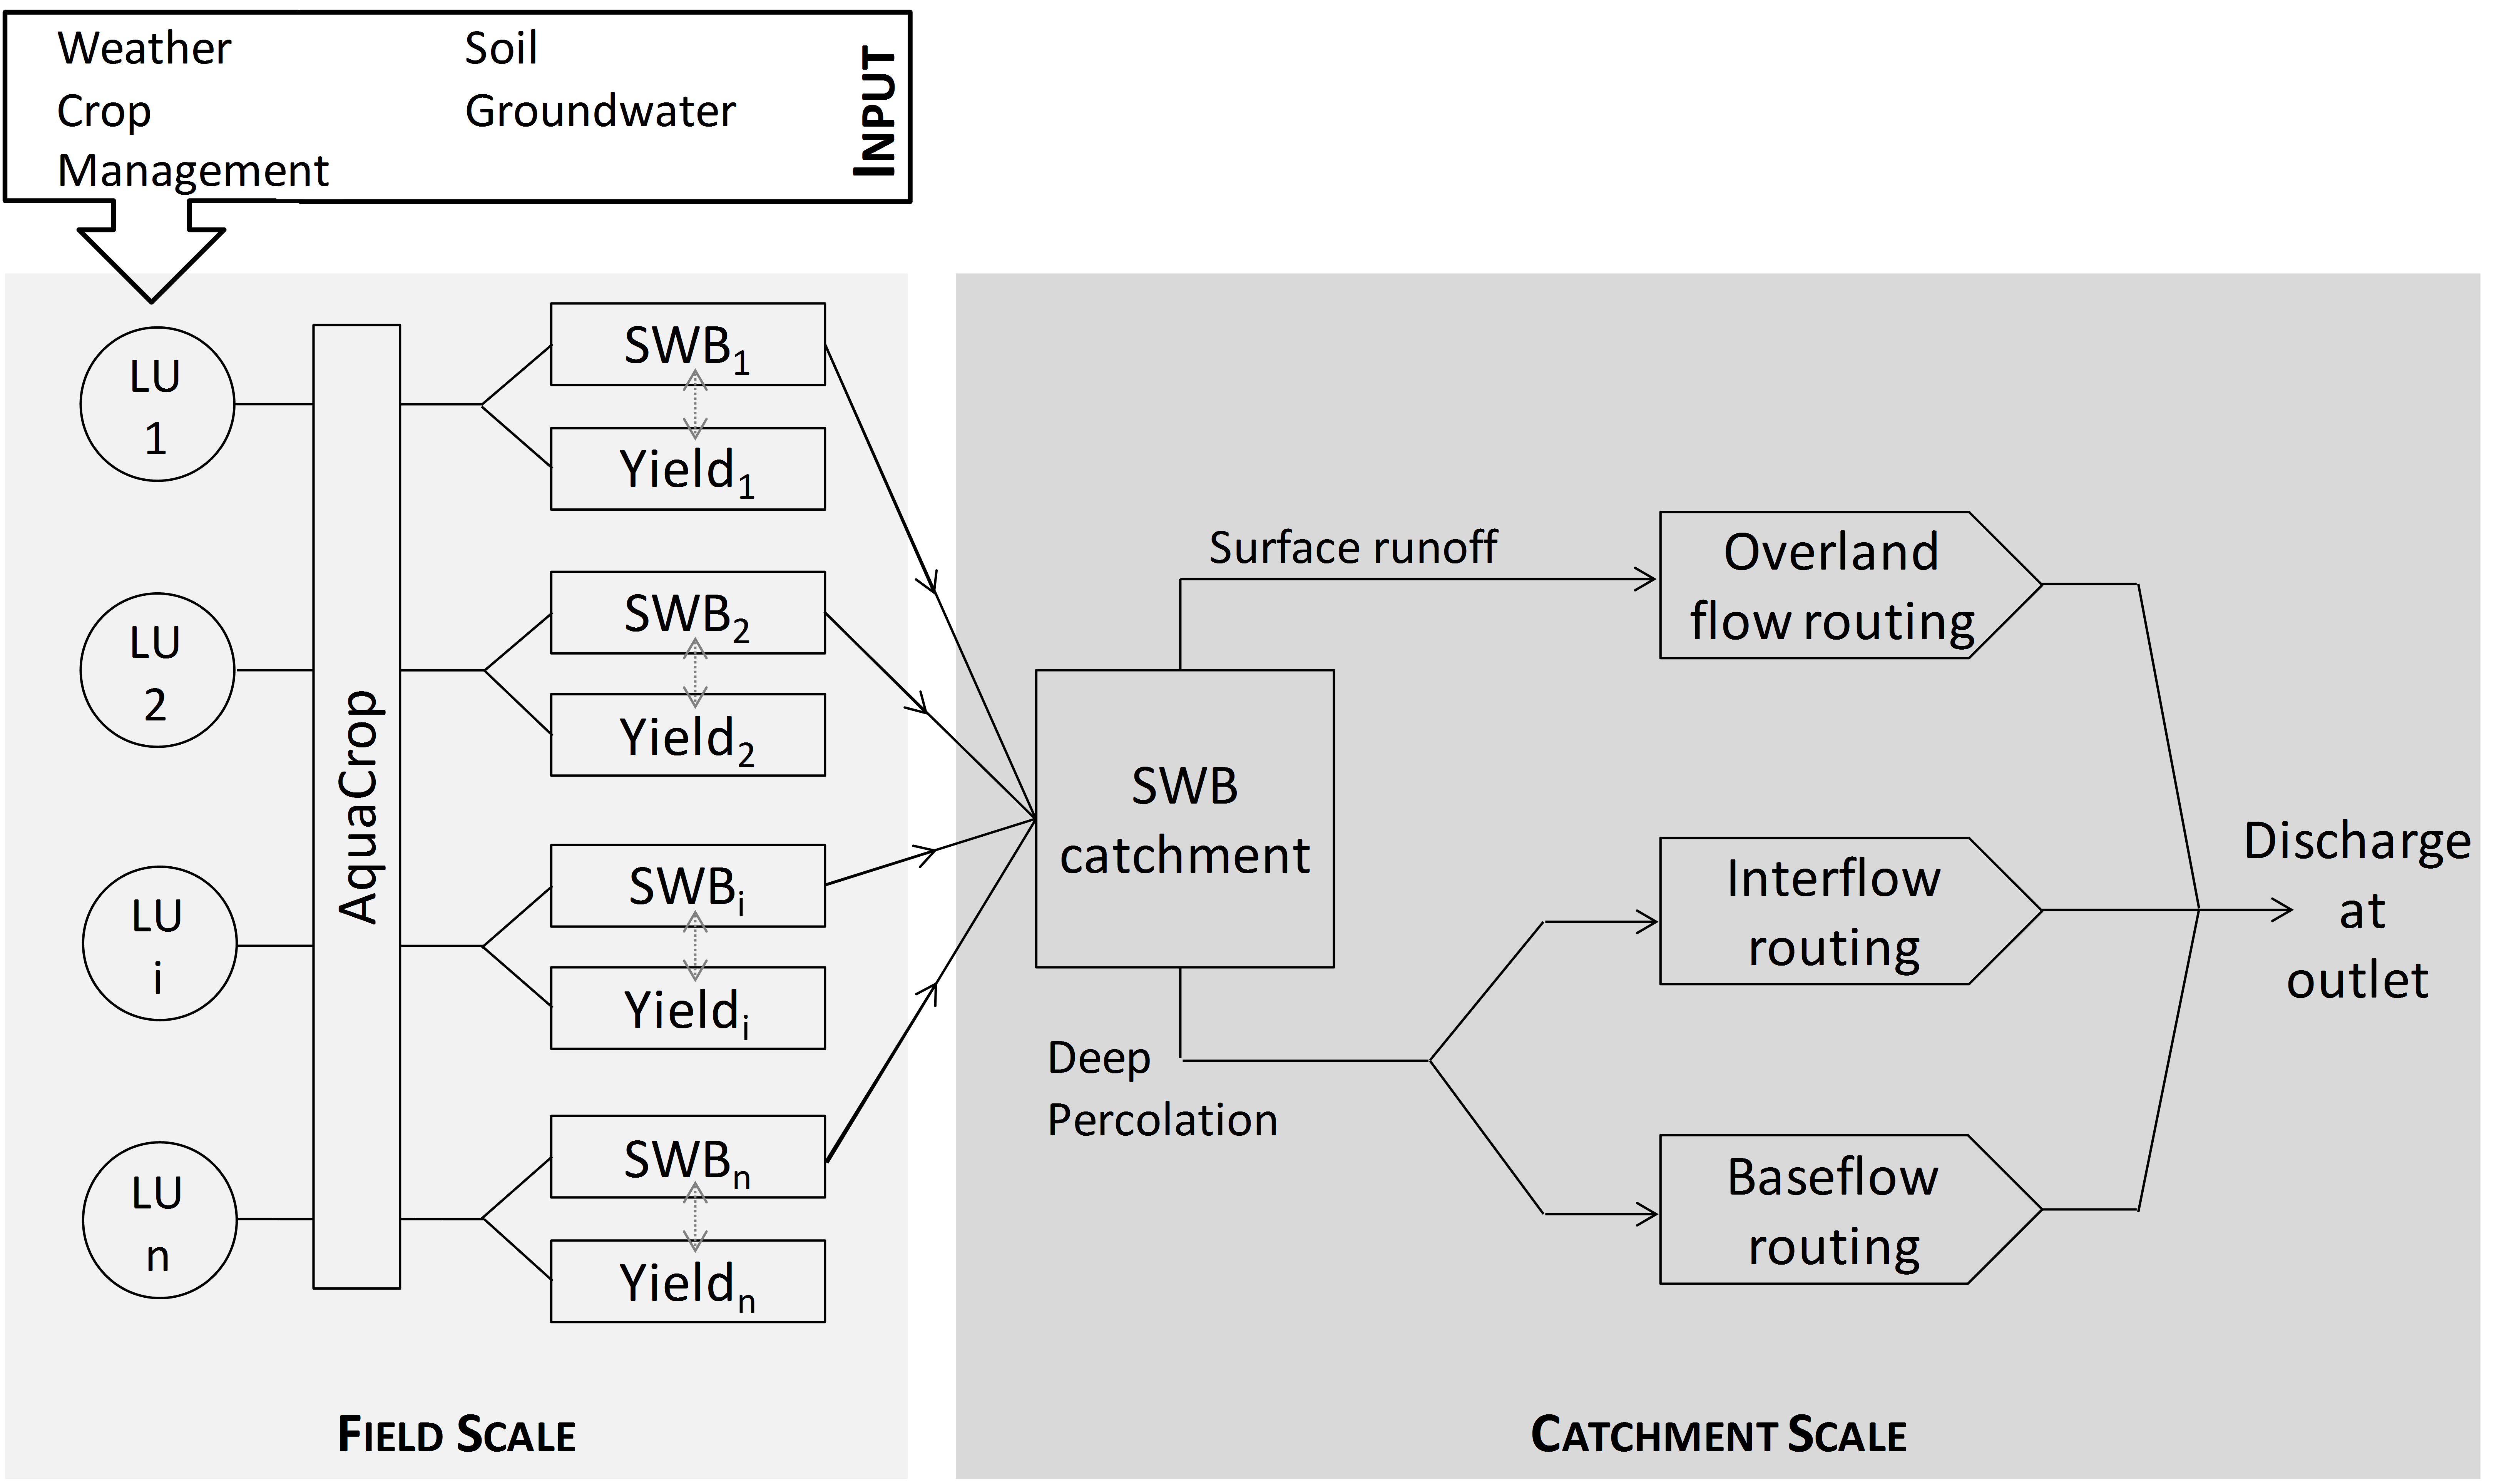
\includegraphics[width=\textwidth]{Flowchart_600dpi.png}
	\caption{Flow chart of the AquaCrop-Hydro model presenting how the AquaCrop soil water balance (SWB) simulations for each individual land unit (LU) are translated into different subflows, which after routing sum up to the total discharge at the catchment outlet.}
	\label{fig:ch6_flowchart}
\end{figure}

\subsubsection{AquaCrop simulation of soil water balance and crop production at field scale}\label{sec:ch6_AC} 
AquaCrop simulates daily crop canopy cover development, transpiration, dry aboveground biomass production, yield and the soil water balance, based on user specified inputs of weather, crop characteristics, soil properties and management practices of the cultivated field (\autoref{fig:ch6_flowchart}). While the soil water balance is calculated for each day of the simulation period, crop development and production simulations are confined to the crop growing period. Being a water-driven model, crop biomass and yield production are simulated proportional to the amount of water transpired by the crop. Transpiration, in its turn, depends on the simulated crop canopy cover and weather conditions. The simulated amount of crop yield per unit evapotranspiration is defined as the crop water productivity (\autoref{sec:ch2_ACsteps}). During this  simulation process, the model accounts for the effect agricultural management(\autoref{sec:ch2_Mgmt}) as well as various abiotic factors, including water stress, temperature stress, soil salinity stress and atmospheric \COtwo concentration (\autoref{sec:ch2_abioticfac}). 

Crop growth and production are adjusted to water stress on the basis of the simulated soil water content in the root zone. Therefore, AquaCrop calculates the daily soil water balance considering incoming (rainfall, irrigation, capillary rise) and outgoing (surface runoff, deep percolation, evaporation, crop transpiration) water fluxes. More information on the calculation of the soil water balance with all its components is presented in \autoref{sec:ch2_SWB}.

Since AquaCrop was developed specifically for herbaceous crops, simulation of LUs with other land use requires specific settings. A bare soil can be simulated by setting the sowing date of the crop after the period of interest. An impervious or urban area can be simulated by bare soil settings in combination with a high curve number (CN) value. An open water surface can be simulated as a bare soil with very low permeability and the presence of soil bunds that ensure water storage in the reservoir. Finally, grassland and forest can be simulated by specifying crop parameters that describe the typical canopy cover development of grass and trees, respectively. Examples for these land uses have been published for alfalfa \parencite{kim2015}, olive trees \parencite{rallo2012}, tea plantations \parencite{elbehri2015} and jatropha \parencite{segerstedt2013}. 

\subsubsection{From field to catchment scale}
Scaling up the field scale AquaCrop results to catchment scale was done as suggested by \textcite{wesseling2006}. After executing AquaCrop for all individual LUs, the different components of the catchment soil water balance (rainfall, irrigation, evaporation, transpiration, surface runoff, capillary rise and deep percolation) and resulting soil water content are simulated as the weighted average of simulation results from all LUs: 
\begin{equation}
 X=\sum_{i=1}^n A_i \cdot x_i
  \label{eq:ch6_SWBcatch}
\end{equation}
where \textit{X} is the soil water balance component or soil water content for the whole catchment, $x_i$ is the soil water balance component or soil water content as simulated for landunit i, $A_i$ is the fraction of the catchment area that is covered by landunit i, and n the number of landunits in the catchment. By adopting this semi-distributed approach, the spatial distribution of each LU within the catchment is disregarded.

\subsubsection{Simulation of catchment hydrology}
The simulated catchment soil water content, deep percolation and surface runoff are used to simulate discharge at the catchment outlet by means of a lumped conceptual routing model, derived from the generalized conceptual model structure by \textcite{willems2014a}. Surface runoff and deep percolation are routed to the outlet by means of three parallel reservoirs (\autoref{fig:ch6_flowchart}). Surface runoff is routed through an overland flow reservoir, while deep percolation reaches the outlet via both an interflow and a baseflow reservoir. Depending on the catchment's behavior, the fraction of deep percolation going to the baseflow ($p_{BF}$) or interflow (1- $p_{BF}$) reservoir can either be considered constant, or can be defined as a function of the simulated soil water content. Each reservoir routes the water according to a linear reservoir equation: 
\begin{equation}
 q_{out}(t)=exp \left(\dfrac{-1}{k}\right) \cdot q_{out}(t-1) + \left( 1-exp \left(\dfrac{-1}{k}\right) \right)\cdot \dfrac{q_{in}(t-1)+q_{in}(t)}{2} 
  \label{eq:ch6_linres}
\end{equation}
where $q_{out}$ and $q_{in}$ are the in- and outflow of the linear reservoir at time step t, and k is the reservoir recession constant. The output of all three reservoirs is finally summed to estimate total discharge at the catchment outlet.

\subsection{Testing AquaCrop-Hydro}
\subsubsection{Study area}	
The Plankbeek stream is located in the sandy loam region of Flanders, Belgium (\autoref{fig:ch6_map}). This area is characterised by a temperate climate with mild winters and cool summers, with rainfall uniformly spread throughout the year. The catchment upstream of the Huise/Plankbeek station (50°54'N, 3°34'E, 17 m a.s.l) covers an area of 4.5 km² and ranges in altitude between 70 m a.s.l. upstream and 17 m a.s.l. at the catchment outlet \parencite{agiv2006}. Silt loam soils dominate the catchment (about 96\%), but sandy loam (about 4\%) soils are found in the upstream area. Soils in the lowest area of the catchment, mainly around the river, are poorly drained \parencite{dov2014}. Agriculture is the dominant land use covering about 94\% of the catchment. The remaining land consists of open water surfaces (0.7\%), deciduous forest (0.2\%) and impervious surface (5\%). While about 18\% of the agricultural land is used as grassland, crops, including winter wheat (20\%), potato (16\%), maize (14\%) and sugar beet (11\%), occupy the majority of the land. Outside the main growing season the majority of fields is left bare, although also grassland (7\%) and cover crops (15 \%) are found \parencite{agiv2014, agiv2001,vlm2014}.
 
 \begin{figure}[tbhp]
	\centering
		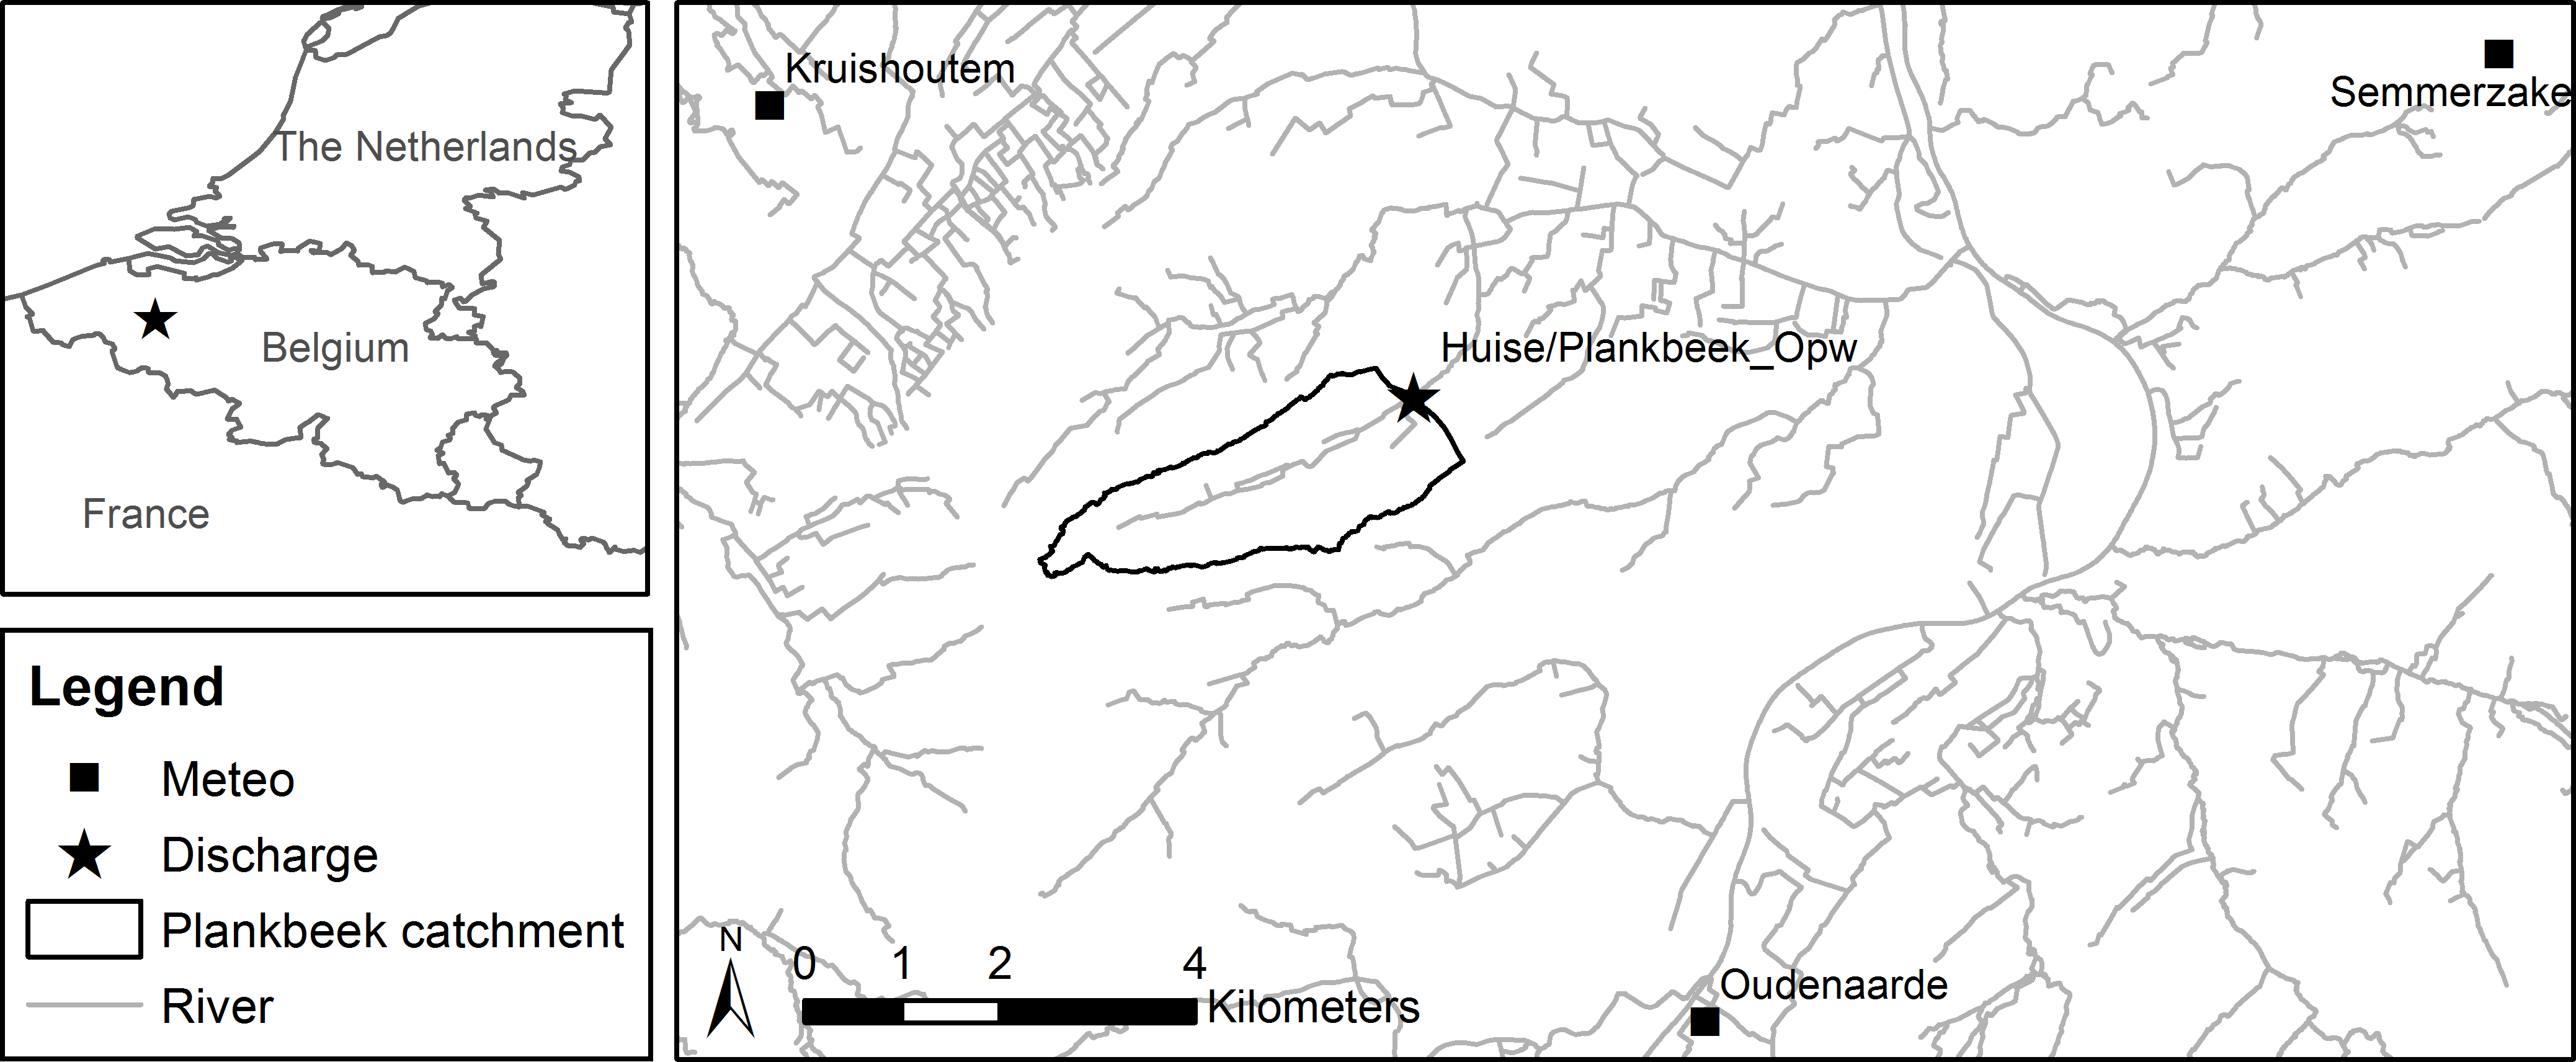
\includegraphics[width=\textwidth]{Map_600dpi.png}
	\caption{Plankbeek catchment with indication of the discharge measurement station at the catchment outlet and nearby meteorological stations. }
	\label{fig:ch6_map}
\end{figure}

\subsubsection{Model input}
AquaCrop-Hydro was executed for a 15-year period from 1/1/2000 to 31/12/2014 using a daily time step. Daily weather data were obtained from nearby meteorological stations (\autoref{fig:ch6_map}) of the Royal Meteorological Institute (KMI). Average catchment rainfall was based on rainfall records of the station of Kruishoutem (50°56'N, 3°31'E, 9 m a.s.l.) and Oudenaarde (50°51'N, 3°37'E, 14 m a.s.l.) using the Thiessen polygon method. Daily minimum and maximum temperature (\Tmin and \Tmax) recorded at the station of Semmerzake (50°56'N, 3°40'E, 37 m a.s.l.) were used. Reference evapotranspiration was calculated with the FAO-Penmann Monteith method using daily data from the station of Semmerzake (\Tmin and \Tmax, minimum and maximum relative humidity, average wind speed) supplemented with measurements of sunshine hours at the station of Melle (50°59'N, 3°49'E, 15 m a.s.l). 

In addition to weather data, AquaCrop-Hydro requires input of crop, soil, groundwater, irrigation and field management characteristics for every simulated LU (\autoref{fig:ch6_flowchart}). For this research, 47 LUs were defined on the basis of soil texture, land use and crop rotation information \parencite{agiv2014,agiv2001,dov2014,vlm2014}. Since land use and the type of cultivated crops was rather stable in the catchment over time, the number and type of LUs were kept constant over the 15-year simulation period. 

Crop parameters (\autoref{tab:ch6_croppar}) for the most prevalent crops, i.e. winter wheat, potato, maize and sugar beet, have already been calibrated for Belgium by \textcite{vanuytrecht2013,vanuytrecht2015, vanuytrecht2014} and could directly be used for this study. The same is true for green bean crop parameters. For other crops, published crop parameters or information from literature \parencite{abrha2012, allen1998, paredes2013, vanuytrecht2013} were used to select crop parameters that match the local cultivation practices and crop varieties. Most attention was paid to canopy and root related parameters, which affect transpiration and the soil water balance most, and to which the model is very sensitive \parencite{vanuytrecht2014b}. Moreover, crops with similar characteristics and growing cycle were assigned the same set of crop parameters. For example, sugar beet parameters were used for simulation of fodder beet, while grass parameters were used for simulation of grass-clover mixtures, clover and other cover crops. This simplification reduced the number of AquaCrop simulations to 31, compared to 47 LUs. Representative sowing dates were selected according to local farming practices. To allow temperature dependent crop canopy development, all simulations were ran in growing degree mode, with the exception of forest and grassland for which a fixed growing cycle length can be assumed. The complete set of crop parameters for each crop is presented in Table A.1.

Default soil parameters (saturated hydraulic conductivity, soil water content at saturation, permanent wilting point and field capacity) were selected from the AquaCrop database for both soil textural classes (i.e. silt loam and sandy loam). Curve number values were selected on the basis of soil type, land use and crop type according to \textcite{usda2007}. Due to lack of information on the groundwater depth in the catchment, capillary rise from the groundwater table was neglected.

Furthermore, according to general practices in Flanders, most farmers do not irrigate and apply sufficient fertilizers to assure non-limiting soil fertility for crop production. LUs with a bare soil, water surface or impervious area were simulated as described above in \autoref{sec:ch6_AC}. Thereby, the saturated hydraulic conductivity of the bottom of the water reservoirs was set to 1 mm/day and the bund heigth to 10 m. The surface runoff curve number of impervious area was set to 98 according to \textcite{usda2007}. AquaCrop simulations started at 1/1/2000 with the initial soil water content at field capacity for all LUs.  

\begin{landscape} 
\begin{table}[htbp]
  	\caption{Overview of simulated crops and key crop parameters. The percentage of the catchment covered by the crop during the main growing season was derived from parcel data for the period 2000-2014. Presented crop parameters include growing cycle length (mat) expressed in growing degree days (GDD) or calendar days (d), maximum canopy cover (\CCx) and corresponding maximum crop coefficient (kcx), as well as maximum effective rooting depth (rtx) and reference harvest index (hio). Crops indicated with + were simulated using the same set of parameters. The complete set of crop parameters is presented in \autoref{tab:AnB_croppar}}
    \resizebox{\linewidth}{!}{
	\begin{threeparttable}
  	\centering
		\begin{tabular}{lrrrrrrrr}
\toprule
\multirow{2}[2]{*}{\textbf{Crop}} & \multicolumn{1}{c}{\textbf{Area}} & \multicolumn{1}{c}{\textbf{Planting}} & \multicolumn{1}{c}{\textbf{mat }} & \multicolumn{1}{c}{\textbf{\CCx }} & \multicolumn{1}{c}{\textbf{kcx}} & \multicolumn{1}{c}{\textbf{rtx}} & \multicolumn{1}{c}{\textbf{hio}} & \multicolumn{1}{c}{\multirow{2}[2]{*}{\textbf{Main reference for crop parameters}}} \\
      & \multicolumn{1}{c}{\textbf{(\%)}} & \multicolumn{1}{c}{\textbf{or regrowth$^\ast$}} & \multicolumn{1}{c}{\textbf{(GDD or d)}} & \multicolumn{1}{c}{\textbf{(-)}} & \multicolumn{1}{c}{\textbf{(-)}} & \multicolumn{1}{c}{\textbf{(m)}} & \multicolumn{1}{c}{\textbf{(\%)}} & \multicolumn{1}{c}{} \\
\midrule
Winter Wheat & \multicolumn{1}{c}{19} & \multicolumn{1}{c}{25 Oct} & \multicolumn{1}{c}{1900 GDD} & \multicolumn{1}{c}{0.92} & \multicolumn{1}{c}{1.1} & \multicolumn{1}{c}{1.5} & \multicolumn{1}{c}{52} & \multicolumn{1}{c}{\parencite{vanuytrecht2013}} \\
Winter Barley  & \multicolumn{1}{c}{1} & \multicolumn{1}{c}{01 Oct} & \multicolumn{1}{c}{1900 GDD} & \multicolumn{1}{c}{0.92} & \multicolumn{1}{c}{1.1} & \multicolumn{1}{c}{1.3} & \multicolumn{1}{c}{33} & \multicolumn{1}{c}{\parencite{abrha2012, vanuytrecht2013}} \\
Maize  & \multicolumn{1}{c}{14} & \multicolumn{1}{c}{25 Apr} & \multicolumn{1}{c}{1200 GDD} & \multicolumn{1}{c}{0.87} & \multicolumn{1}{c}{1.05} & \multicolumn{1}{c}{1.1} & \multicolumn{1}{c}{52} & \multicolumn{1}{c}{\parencite{vanuytrecht2015,vanuytrecht2014}} \\
Sugar beet & \multicolumn{1}{c}{11} & \multicolumn{1}{c}{15 Apr} & \multicolumn{1}{c}{1850 GDD} & \multicolumn{1}{c}{0.98} & \multicolumn{1}{c}{1.1} & \multicolumn{1}{c}{1} & \multicolumn{1}{c}{70} & \multicolumn{1}{c}{\parencite{vanuytrecht2015}} \\
      + Fodderbeet &       &       &       &       &       &       &       &  \\
Potato & \multicolumn{1}{c}{15} & \multicolumn{1}{c}{25 Apr} & \multicolumn{1}{c}{1850 GDD} & \multicolumn{1}{c}{1} & \multicolumn{1}{c}{1.1} & \multicolumn{1}{c}{0.6} & \multicolumn{1}{c}{90} & \multicolumn{1}{c}{\parencite{vanuytrecht2015}} \\
Green beans & \multicolumn{1}{c}{1} & \multicolumn{1}{c}{1 Jun} & \multicolumn{1}{c}{870 GDD} & \multicolumn{1}{c}{1} & \multicolumn{1}{c}{1.1} & \multicolumn{1}{c}{0.6} & \multicolumn{1}{c}{22} & \multicolumn{1}{c}{\parencite{vanuytrecht2013}} \\
Peas  & \multicolumn{1}{c}{6} & \multicolumn{1}{c}{01 Apr} & \multicolumn{1}{c}{945 GDD} & \multicolumn{1}{c}{0.9} & \multicolumn{1}{c}{1.1} & \multicolumn{1}{c}{0.5} & \multicolumn{1}{c}{34} & \multicolumn{1}{c}{\parencite{paredes2013}} \\
Carrot & \multicolumn{1}{c}{4} & \multicolumn{1}{c}{15 May} & \multicolumn{1}{c}{1850 GDD} & \multicolumn{1}{c}{0.95} & \multicolumn{1}{c}{0.95} & \multicolumn{1}{c}{0.6} & \multicolumn{1}{c}{60} & \multicolumn{1}{c}{\parencite{allen1998,vanuytrecht2013}} \\
      + Chicory &       &       &       &       &       &       &       &  \\
Grassland & \multicolumn{1}{c}{18} & \multicolumn{1}{c}{15 Mar} & \multicolumn{1}{c}{215-365 \si{d}$^\ast\ast$} & \multicolumn{1}{c}{0.9} & \multicolumn{1}{c}{0.85} & \multicolumn{1}{c}{0.6} & \multicolumn{1}{c}{85} & \multicolumn{1}{c}{\parencite{allen1998}} \\
      + Clover &       &       &       &       &       &       &       &  \\
      + Grass-clover  &       &       &       &       &       &       &       &  \\
      + Cover crop &       &       &       &       &       &       &       &  \\
Decidious Forest & \multicolumn{1}{c}{0.2} & \multicolumn{1}{c}{15 Mar} & \multicolumn{1}{c}{231 \si{d}} & \multicolumn{1}{c}{0.9} & \multicolumn{1}{c}{0.95} & \multicolumn{1}{c}{1.5} & \multicolumn{1}{c}{-} & \multicolumn{1}{c}{\parencite{allen1998}} \\
\bottomrule				
    	\end{tabular}%
    	\begin{tablenotes}
        \item[$\ast$] Sowing or planting for annual crops, regrowth for perennials
        \item[$\ast\ast$] Growing cycle length varies depending on the temporary or permanent character of the grassland 
    	\end{tablenotes}
        \end{threeparttable}
              }
  \label{tab:ch6_croppar}%
\end{table}%
\end{landscape}
 
The catchment soil water balance and soil water content were calculated using \autoref{eq:ch6_SWBcatch}, with $A_i$ being the average relative area of each LU as calculated from parcel data for the period 2000-2014 \parencite{vlm2014}. Crops that occupied on average less than 0.5\% of the agricultural area were excluded from simulation. Instead, the agricultural LUs containing these non-simulated crops were assigned the weighted average results of other agricultural LUs with the same soil type. Due to the variation of rooting depth during the growing season and between different crops, the catchment soil water content was calculated from the soil water content in the first 2 m of soil of each LU. 

Furthermore, deep percolation was split into a baseflow and interflow fraction with \autoref{eq:ch6_pbf} assuming that baseflow decreases linearly when the soil water content varies between field capacity and the highest soil water content of the simulation period:
\begin{equation}
 p_{BF}(t)=p_{BF,FC} + \dfrac{SWC(t)-SWC_{FC}}{SWC_{max}-SWC_{FC}} \cdot \left(p_{BF,max} -p_{BF,FC}\right) 
  \label{eq:ch6_pbf}
\end{equation}
where $p_{BF}(t)$ (-) is the fraction of deep percolation that goes to the baseflow reservoir ($p_{BF}$) at time step t when the total soil water content in the first 2 m of soil is $SWC(t)$ (mm), $p_{BF,FC}$ is $p_{BF}$ when the soil water content is at field capacity ($SWC_{FC}$), and $p_{BF,max}$ is $p_{BF}$ when the soil water content is at its highest simulated value ($SWC_{max}$). 

Field capacity was chosen as the lower threshold, as AquaCrop only simulates deep percolation if the soil water content is above field capacity. The $p_{BF}$ thresholds ($p_{BF,FC}$ and $p_{BF,max}$) were determined during the hydrological model calibration process, together with the three recession constants for baseflow, interflow and overland flow.

\subsubsection{Model evaluation}
AquaCrop-Hydro simulations of discharge were evaluated using daily average discharge observations from the station Huise/Plankbeek\_Opw \parencite{vmm2015} located at the catchment outlet (\autoref{fig:ch6_map}). Since no discharge observations were available for 1/1/2000-8/6/2002, this was considered as the warming-up period for the model. Hydrological model parameters (three recession constants, $p_{BF,max}$ and $p_{BF,FC}$) were calibrated for the period 9/6/2002 to 15/8/2010 (about 8 years), while model simulations were validated for 15/8/2010 to 31/12/2014 (about 4.5 years). The 400 days (110 in calibration and 290 in validation period) for which discharge data were missing were excluded when comparing model results with the observations. 

The routing model was calibrated according to the step-wise procedure (`VHM approach') by \textcite{willems2014a} which relies on information about the catchment runoff response to the meteorological inputs derived after time series processing using WETSPRO \parencite{willems2009}. Thereby the observed discharge is separated into different subflows (baseflow, interflow and overland flow) by means of a generalized Chapman-filter. During the subflow separation process, the recession constants (k) of the subflows are identified by analyzing the slopes in different parts of the recession limbs of the hydrographs or flow time series during long dry periods. The second filter parameter (w) is selected by optimizing the height of the subflow during a recession period as explained by \textcite{willems2009}. This parameter can be either chosen to be constant or variable depending on the total discharge. Finally, a backward time shift is applied to compensate for the delayed subflow filter result in comparison with the total flow. \autoref{tab:ch6_wetspropar} presents the filter settings, defined by visual inspection of the time-series, to separate daily average discharge at the outlet of the Plankbeek catchment into subflows. 

\begin{table}[htbp]
  	\caption{WETSPRO parameters for filtering average daily discharge measurements at Huise/Plankbeek\_Opw station for period 9/6/2002-31/12/2014. Discharge was filtered into baseflow, interflow and remaining overland flow.}
    %\resizebox{\textwidth}{!}{
\begin{tabular}{lccc}
\toprule
\textbf{Filter parameter} & \textbf{Baseflow} & \textbf{Interflow} & \textbf{Overland flow} \\
\midrule
Recession constant k (d) & 35    & 2     & 0.3 \\
Time shift (d) & 3     & 0     &  \\
Filter parameter w (-) & Exponential & Constant &  \\
      & 0.2 to 0.65 & 0.6   &  \\
\bottomrule
\end{tabular}%
%}
  \label{tab:ch6_wetspropar}%
  \end{table}

Values for the AquaCrop-Hydro recession constants were directly obtained from the WETSPRO filter (\autoref{tab:ch6_wetspropar}). The $p_{BF}$ thresholds ($p_{BF,FC}$ and $p_{BF,max}$) in \autoref{eq:ch6_pbf} were calibrated to the filtered daily baseflow to interflow fraction as a function of the simulated soil water content on that day. Evaluation of AquaCrop-Hydro’s river flow simulation included comparison of simulated and observed cumulative water volumes, total discharge and subflows. Evaluation considered daily time steps, as well as aggregated time steps of 10 days or one month. 

In addition, AquaCrop-Hydro simulations of seasonal dry crop yield were evaluated against observations of average crop productivity for the period 2000-2013 in the sandy loam region, which covers a large part (5130 km2) of central Belgium \parencite{fodeconomie2014}. Crop yield simulations were evaluated for maize, winter wheat, winter barley, potato, sugar beet, green beans and peas, covering over 70\% of the agricultural land of the catchment. Fresh weight yield observations were corrected using typical values of crop's dry matter content at harvest: 25\% for potato, 19\% for sugar beet, 15\% for green beans and 25\% for peas.

Model evaluation was based on graphical displays as well as the four statistical indicators presented in Box \ref{box:ch2_Eval}: \Rsq, RRMSE and EF and RME. 

\section{Results}
\subsection{Hydrological model parameters}
\autoref{tab:ch6_hydropar} shows the five hydrological model parameters as calibrated for the Plankbeek catchment. The calibrated deep percolation parameters resulted in a good match between the observed and simulated baseflow-interflow proportion. Comparison for all days with deep percolation resulted in a high \Rsq of 0.86. The baseflow and interflow recession constants were taken equal to values obtained when applying the WETSPRO filter (\autoref{tab:ch6_wetspropar}). The calibrated overland flow recession constant resulted in a 7 times faster overland flow recession as compared to interflow.

\begin{table}[htbp]
\begin{tabularx}{\textwidth}{Xc}
  	\caption{Model parameters for the lumped conceptual hydrological model of AquaCrop-Hydro}\\
\toprule
\textbf{Deep percolation parameters} & \textbf{Value (-)} \\
\midrule
Baseflow fraction for soil at field capacity ($p_{BF,FC}$) & 0.88 \\
Baseflow fraction for maximum soil water content ($p_{BF,max}$) & 0.4 \\
\textbf{Routing parameters} & \textbf{Value (d)} \\
\midrule
Recession constant baseflow ($k_{BF}$) & 35 \\
Recession constant interflow ($k_{IF}$) & 2 \\
Recession constant overland flow ($k_{OF}$) & 0.3 \\
\bottomrule
\end{tabularx}%
  \label{tab:ch6_hydropar}%
  \end{table}

\subsection{Model performance}
\subsubsection{Crop production}
Average simulated crop production matched well with the average crop yield reported for the catchment region (\autoref{tab:ch6_YieldPerf}). The absolute deviation between observed and simulated yield was not more than 0.4 t/ha, except for maize and winter wheat. Moreover, RRMSE values, summarizing model performance for a year-by-year comparison of simulated and observed yield, ranged between 7\% and 37\%. Excellent model performance was found for winter barley, while the model performed rather poorly for winter wheat. 

\begin{table}[htbp]
  \centering
  	\caption{Comparison of observed and simulated average crop yield (t dry matter/ha) for the Plankbeek catchment during the period 2000-2013, with corresponding relative root-mean-square error (rRMSE). }
    %\resizebox{\linewidth}{!}{
\begin{tabular}{lccccc}
\toprule
      & \multicolumn{2}{c}{\textbf{Observed}} & \multicolumn{2}{c}{\textbf{Simulated}} & \multicolumn{1}{c}{\textbf{RRMSE}} \\
      & \multicolumn{2}{c}{\textbf{yield \si{t/ha}}} & \multicolumn{2}{c}{\textbf{yield \si{t/ha}}} & \textbf{(\%)} \\
      & Average & SD    & Average & SD    & \multicolumn{1}{l}{} \\
\midrule
Maize & 11.975 & 0.621 & 10.518 & 0.647 & 14.9 \\
Winter wheat  & 8.590 & 0.582 & 11.425 & 1.040 & 36.5 \\
Winter barley  & 7.901 & 0.543 & 8.160 & 0.401 & 7.1 \\
Potato & 11.932 & 1.036 & 11.753 & 2.861 & 23.0 \\
Sugar beet & 13.740 & 1.332 & 14.126 & 1.251 & 12.1 \\
Green beans & 1.940 & 0.208 & 1.742 & 0.307 & 22.4 \\
Peas  & 1.964 & 0.202 & 1.984 & 0.470 & 25.4 \\
\bottomrule
\end{tabular}%

  \label{tab:ch6_YieldPerf}%
  \end{table}

\subsubsection{Soil water balance}
\autoref{tab:ch6_Wabal} presents the simulated catchment soil water balance for the complete simulation period. About 65\% of the rainfall is simulated to leave the catchment as evapotranspiration. The remaining rainfall mostly percolates to the groundwater (27\%), or leaves the catchment through surface runoff (7.5\%). Building up of stored water in the catchment during the simulation period is minimal (0.2\% of rainfall). The soil water balance was not fully closed, but the error of 9 mm (0.1\%) over a period of 15 years was negligible. This error was caused by the fact that AquaCrop output for the soil water balance components is rounded off to one decimal. These rounding off errors accumulated by summing up daily values over the 15 year simulation period. 

\begin{table}[htbp]
  \centering
  	\caption{Simulated catchment water balance for the simulation period 1/1/2000-31/12/2014. Positive/negative values present a net inflow/outflow. Water storage includes both soil water storage and water storage in surface water reservoirs.}
    %\resizebox{\textwidth}{!}{
\begin{tabular}{lcc}
\toprule
\textbf{Water component} & \textbf{Net flux (mm)} & \textbf{\% of rainfall} \\
\midrule
Rainfall & 12776.2 & 100.0 \\
Evaporation & -4033.4 & -31.6 \\
Transpiration  & -4347.9 & -34.0 \\
Deep percolation  & -3457.6 & -27.1 \\
Surface runoff  & -958.9 & -7.5 \\
Water storage  & 30.5  & 0.2 \\
Total & 8.9   & 0.1 \\
\bottomrule
\end{tabular}%
%}
  \label{tab:ch6_Wabal}%
  \end{table}


\subsubsection{Cumulative water volume}
The AquaCrop-Hydro model simulates the total cumulative water volume with a small underestimation of about 7\% (\autoref{tab:ch6_FlowBal}). As it is clear from \autoref{fig:ch6_cumflow}, this underestimation at the end of the simulation period is the result of underestimation during the calibration period (14.5\%), which is partly compensated by overestimation during the validation period (12\%). Lower overland flow volumes are simulated by the model compared to the filter results (about 24\% difference), while the total volume of deep percolation, reaching the outlet via baseflow and interflow, is only lower by about 4\%. Furthermore, calibration of the deep percolation parameters (\autoref{tab:ch6_hydropar}) resulted in good simulations of baseflow (2.5\% difference) and interflow volumes (about 10\% difference). 

\begin{table}[htbp]
  	\caption{Cumulative water volumes for the evaluation period 6/9/2002-31/12/2014 (400 missing days excluded), together with the corresponding relative model error. Values marked with * are observations obtained by the subflow filter. The sum of simulated baseflow and interflow is equal to the simulated deep percolation (DP), while overland flow is equal to simulated surface runoff (RO).}
    %\resizebox{\linewidth}{!}{
\begin{tabular}{lcccc}
\toprule
\multirow{2}[2]{*}{\textbf{}} & \textbf{Observed} & \textbf{Simulated} & \textbf{Error} & \textbf{RME} \\
      & \textbf{(mm)} & \textbf{(mm)} & \textbf{(mm)} & \textbf{(\%)} \\
\midrule
Total discharge & 3509 & 3266  & 243   & 6.9 \\
Baseflow + Interflow (=DP) & 2668$^\ast$ & 2560  & 109   & 4.1 \\
Baseflow & 2081$^\ast$ & 2029  & 52    & 2.5 \\
Interflow & 587$^\ast$  & 531   & 56    & 9.6 \\
Overland flow (=RO) & 932$^\ast$  & 707   & 225   & 24.2 \\
\bottomrule
\end{tabular}%
%}
  \label{tab:ch6_FlowBal}%
  \end{table}

 \begin{figure}[tbhp]
	\centering
		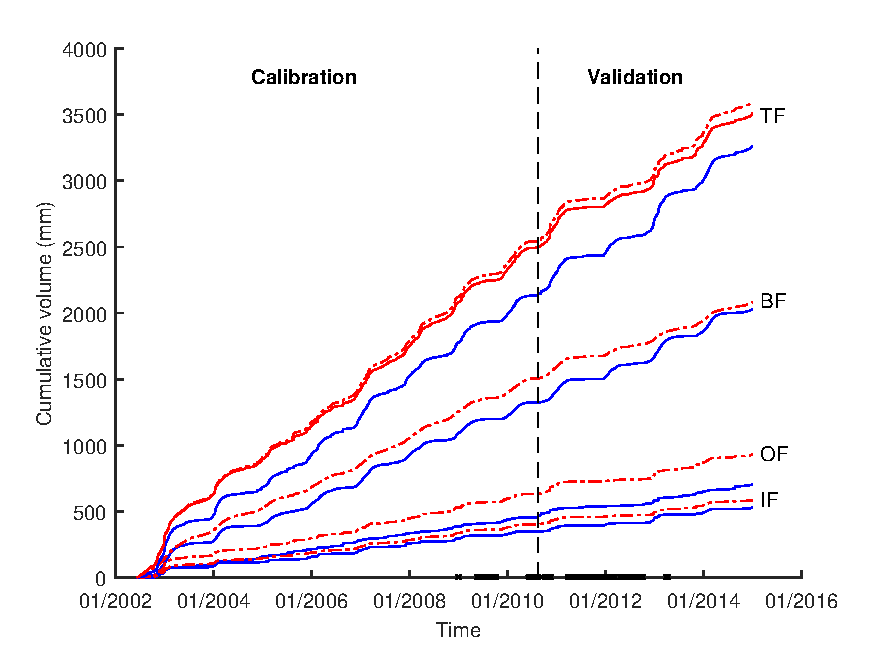
\includegraphics[width=\textwidth]{CumFlow_600dpi.pdf}
	\caption{Simulated versus observed cumulative water volumes of total discharge (TF), baseflow (BF), interflow (IF) and overland  flow (OF) during the evaluation period 6/9/2002-31/12/2014. Simulated values are presented by a full line. Dotted lines display observed values, while dashed lines show values obtained by the subflow filter. Time steps with missing observations, excluded from the cumulative totals (for both observations and simulations), are marked on the time axis with x.}
	\label{fig:ch6_cumflow}
\end{figure}


\subsubsection{Daily discharge}
\autoref{fig:ch6_totalflow}  shows that AquaCrop-Hydro was capable to simulate the flow dynamics at the catchment outlet. Average daily discharge was simulated with an EF of 0.64 and \Rsq of 0.67 for the complete evaluation period (\autoref{tab:ch6_FlowPerf}). Performance was slightly better for the calibration period compared to the validation period. Despite the satisfactory simulation of total discharge, statistics reveal unsatisfactory performance for baseflow and overland flow, while the best match between simulation results and filtered subflow were obtained for interflow.

\begin{table}[htbp]
  	\caption{Performance indicators for simulation of average daily total discharge and corresponding subflows at the outlet of the Plankbeek catchment during the calibration, validation and complete evaluation period. `n' is the number of days for which model performance was evaluated, \Rsq is the coefficient of determination and EF the Nash-Sutcliffe model efficiency. }
    %\resizebox{\linewidth}{!}{
\begin{tabular}{lccccccccc}
\toprule
      & \multicolumn{3}{c}{Calibration} & \multicolumn{3}{c}{Validation} & \multicolumn{3}{c}{Calibration + Validation} \\
      & n     & \Rsq    & EF    & n     & \Rsq     & EF    & n     & \Rsq     & EF\\
\midrule
\multicolumn{1}{l}{Total discharge} & 2879  & 0.68  & 0.66  & 1310  & 0.62  & 0.61  & 4189  & 0.65  & 0.64 \\
\multicolumn{1}{l}{Baseflow} & 2879  & 0.74  & -0.04 & 1310  & 0.71  & -0.45 & 4189  & 0.69  & -0.16 \\
\multicolumn{1}{l}{Interflow} & 2879  & 0.74  & 0.69  & 1310  & 0.63  & 0.60   & 4189  & 0.70   & 0.65 \\
\multicolumn{1}{l}{Overland flow} & 2879  & 0.45  & 0.44  & 1310  & 0.50   & 0.50   & 4189  & 0.47  & 0.47 \\
\bottomrule
\end{tabular}%
%}
  \label{tab:ch6_FlowPerf}%
  \end{table}

\begin{landscape} 
 \begin{figure}[tbhp]
	\centering
		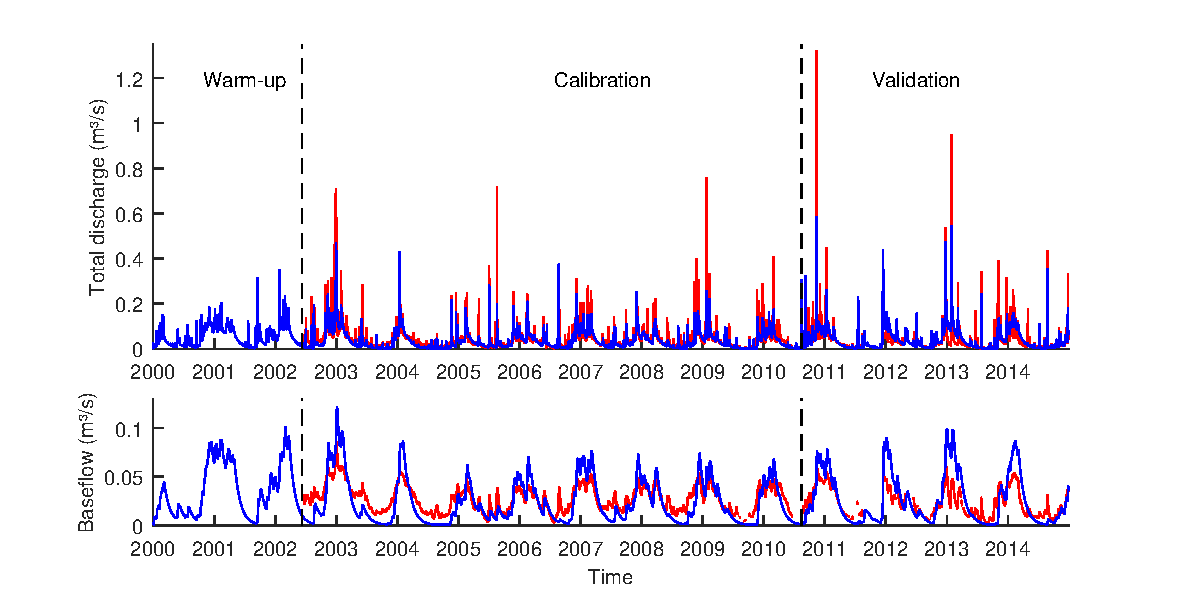
\includegraphics[trim=1.2cm 0cm 1cm 1cm, clip=true, width=19.2cm]{TotalFlow_600dpi.pdf}
	\caption{Simulated (blue line) versus observed or filtered (red line) average daily total discharge (top) and baseflow (bottom) at the outlet of the Plankbeek catchment for the simulation period 1/1/2000-31/12/2014. Dashed lines separate the simulation period in the warm-up, calibration and validation periods.}
	\label{fig:ch6_totalflow}
\end{figure}
\end{landscape}
  
The model output error for total discharge can be largely explained by the lower model performance for overland flow, with an efficiency of 0.44 to 0.5; although potential inaccuracies in the structure and application of the subflow filter should be taken into account as well. \autoref{fig:ch6_totalflow} indicates that peak flow events, which are mainly dominated by quick flow processes such as overland flow, were underestimated by AquaCrop-Hydro. Operating at a daily time step, AquaCrop-Hydro neglects the effect of rainfall intensity on surface runoff generation. As shown in \autoref{fig:ch6_OFprob}, two similar rainfall events, occurring when the soil was at field capacity, led to simulation of a similar surface runoff event. By contrast, the filtered overland flow showed a different response to both rainfall events, most likely because of the differences in rainfall distribution over the day. 

 \begin{figure}[tbhp]
	\centering
		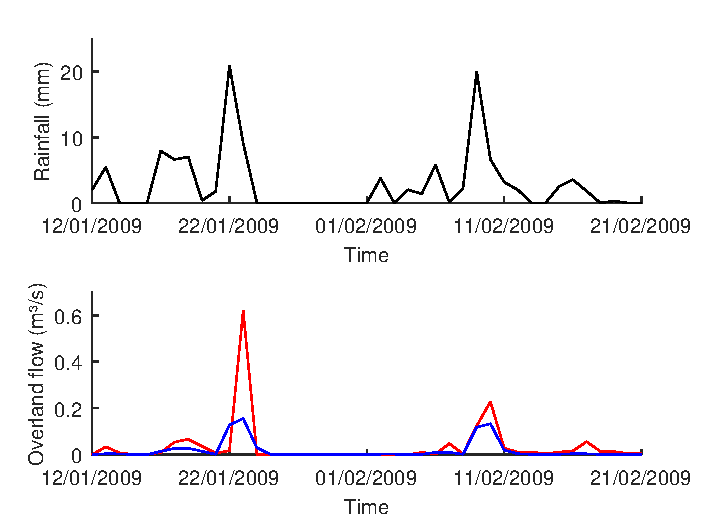
\includegraphics[width=10cm]{OFprob_600dpi.pdf}
	\caption{Two similar rainfall events (top) result in a similar response of simulated daily overland flow (bottom, blue line), but a different response of average daily filtered overland flow (bottom, red line). }
	\label{fig:ch6_OFprob}
\end{figure} 

Furthermore, \autoref{fig:ch6_totalflow} indicates that underestimation of total discharge during low flow periods, dominated by baseflow, was another important source of error. Also performance statistics show low model efficiency for baseflow (-0.45 to -0.04), despite the good \Rsq values (\autoref{tab:ch6_FlowPerf}). Particularly during dry summers in the calibration period (2002-2004, 2008-2009) the underestimation of baseflow was remarkable. During these dry periods, \autoref{fig:ch6_BFprob} shows how simulated deep percolation completely falls to zero as rainfall is insufficient to bring the soil water content above field capacity. By contrast, baseflow observations do present a reaction to rainfall events in summer periods. This could be due to the presence of saturated soils in the catchment, which immediately drain after a rainfall event. However, such events were not considered in the model, as AquaCrop-Hydro was executed with the assumption that there is no shallow groundwater table in the catchment.

 \begin{figure}[tbhp]
	\centering
		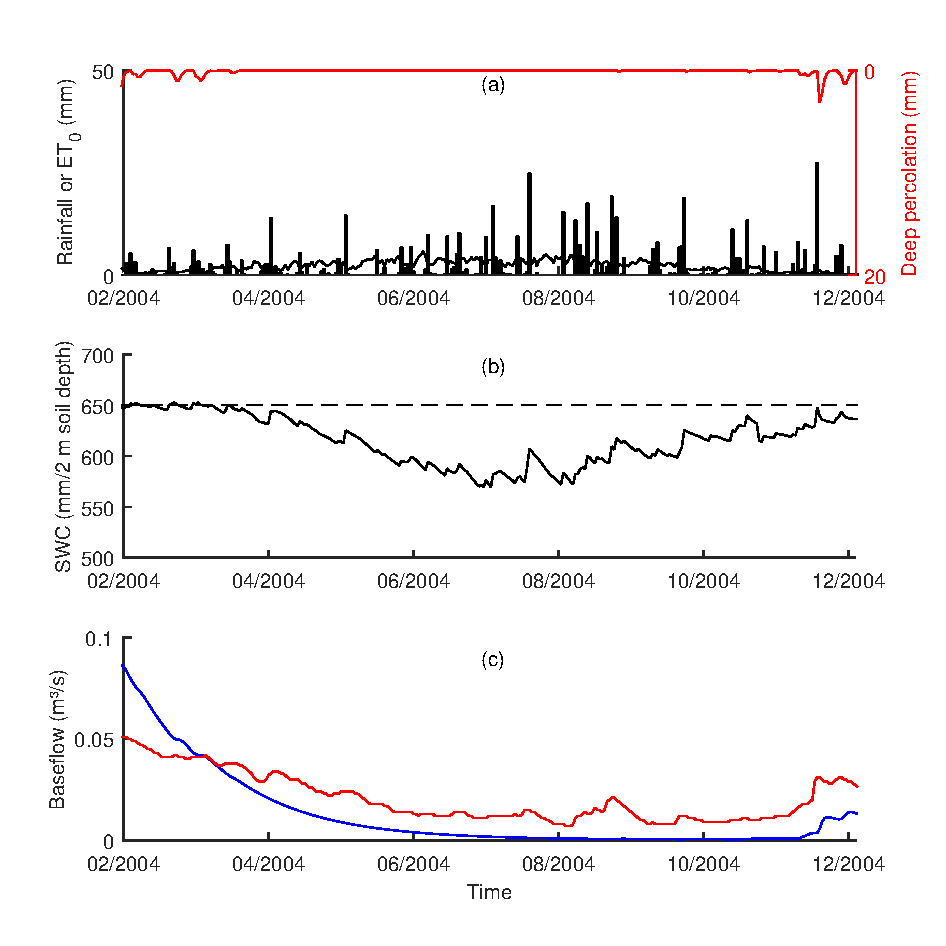
\includegraphics[width=\textwidth]{BFprob_600dpi.pdf}
	\caption{(a) Simulated rainfall (bars), reference evapotranspiration (\ETo) (black line) and deep percolation (red line) with (b) corresponding soil water content, and (c) resulting observed (red line) versus simulated (blue line) baseflow. Dashed line in b indicates the soil water content at field capacity. }
	\label{fig:ch6_BFprob}
\end{figure}  

Finally, \autoref{fig:ch6_totalflow} shows that particularly during wet periods in the validation period, baseflow and consequently total discharge were overestimated. This is also reflected by the negative EF value for baseflow during validation (-0.45). The overestimation of baseflow appears to be linked to the underestimation of overland flow during wet periods with intensive rainfall. Since the baseflow overestimation partly compensated the underestimation during the calibration period, the final baseflow volume at the end of the simulation period matched the observed volume well (\autoref{tab:ch6_FlowBal} and \autoref{fig:ch6_cumflow}). 

\subsubsection{Aggregated flow volumes}
\autoref{tab:ch6_FlowPerfAggr} shows that AquaCrop performs better to simulate monthly or 10-daily flow volumes, compared to daily discharge. Model efficiency for simulation of total discharge increases from 0.64 at daily basis to 0.82 for 10-daily and monthly flow volumes. 

\begin{table}[htbp]
\centering
  	\caption{Performance indicators for simulation of average daily total discharge at the outlet of the Plankbeek catchment during the complete evaluation period 6/9/2002-31/12/2014, when evaluated at daily, 10-daily or monthly basis. `n' is the number of daily, 10-daily or monthly periods for which model performance was evaluated, \Rsq is the coefficient of determination and EF the Nash-Sutcliffe model efficiency.}
    %\resizebox{\textwidth}{!}{
\begin{tabular}{rccc}
\toprule
      & n     & \Rsq    & EF \\
\midrule
\multicolumn{1}{l}{Daily total discharge} & 4189  & 0.65  & 0.64 \\
\multicolumn{1}{l}{10-daily total discharge } & 436   & 0.83  & 0.82 \\
\multicolumn{1}{l}{Monthly total discharge} & 147   & 0.85  & 0.82 \\
\bottomrule
\end{tabular}%
%}
  \label{tab:ch6_FlowPerfAggr}%
  \end{table}


\section{Discussion}
\subsection{Model approach and performance}
This study shows that AquaCrop-Hydro combines the benefits and functionality of the physically based AquaCrop model and a parsimonious conceptual hydrological model in order to upscale simulation of water availability from an individual field to a larger agricultural catchment. Moreover, AquaCrop-Hydro has low data and calibration requirements thanks to selection of simple transparent sub-models. Also, AquaCrop-Hydro performs well to simulate crop production and discharge at the catchment outlet. Considering all this, AquaCrop-Hydro displays an optimal balance between model applicability, transparency and accuracy for simulation of crop (water) productivity and water availability in agricultural catchments. With these key features, AquaCrop-Hydro tackles many of the limitations of previously developed agro-hydrological model combinations that were identified in the introduction section. 

The major strength of AquaCrop-Hydro is its low requirements for easily obtainable input or calibration data, due to the limited requirements of its two sub-models. AquaCrop, by its nature, requires a limited amount of input data and parameters, which can be easily obtained from field observations, agricultural statistics or literature \parencite{vanuytrecht2014a}. Moreover, crop parameters are available for several crops as the AquaCrop model has been calibrated already for more than 30 crops. These include widely cultivated crops such as maize, barley, wheat and cotton \parencite{abrha2012, andarzian2011, garciavila2009, heng2009}, but also underutilized crops such as quinoa, teff and bambara groundnut \parencite{geerts2009a, mabhaudhi2014, tsegay2012}. Additional parameter sets for new crops are published every year. Also, for soil parameters and management inputs, the user can rely on default settings of AquaCrop, as illustrated by the above case-study. 

Furthermore, the hydrological model parameters of AquaCrop-Hydro can be easily obtained from time series of river discharge observations. Such time series are commonly available, even in data scarce regions, at least for one station (e.g. downstream the catchment) or for a neighbouring catchment. In addition, these time series do not need to cover the complete simulation period, but should be long enough to cover at least some quick and slow runoff events. Furthermore, as the model focuses on estimating water availability, one does not need flow data with very small time resolution. A time step of one day, as considered in this study, would be sufficient. For larger catchments one could even consider larger time steps. 

Due to these limited data requirements AquaCrop-Hydro is applicable to various agricultural catchments, even in data-scarce regions. This is supported by the fact that AquaCrop has been  applied to different cropping systems all around the world \parencite{vanuytrecht2014a}, including data scarce regions in developing countries like Ethiopia \parencite{abrha2012, tsegay2012}, Burkina Faso \parencite{wellens2013}, Iran \parencite{andarzian2011}, Bolivia \parencite{geerts2009a} and Nepal \parencite{shrestha2013}. Also, model comparison studies mention that AquaCrop is easier to apply in data-scarce regions as compared to other crop models such as CropSyst, WOFOST and CERES \parencite{abisaab2015, castanedavera2015,todorovic2009}. Furthermore, conceptual models defined according to the top-down concept by \textcite{willems2014a} (`VHM approach'), which was also implemented in AquaCrop-Hydro, were already applied to data-scarce areas in countries such as Ecuador \parencite{moraserrano2013}, China \parencite{liu2011}, Uganda \parencite{nyekoogiramoi2010}, Kenya and Ethiopia \parencite{taye2011}. In addition, the generalized model structure of the routing model allows flexible adjustment of AquaCrop-Hydro to variable catchment conditions. The interflow routing component, for example, can easily be discarded if this flow component appears negligible. 

Calibration of agro-hydrological models is often challenging. The lack of transparent calibration procedures tends to cause problems to identify parameter values, especially for overparameterized models with strong interaction between different model parameters \parencite{andreassian2012, beven2006}. By contrast, AquaCrop-Hydro contains a limited number of parameters to be calibrated using a transparent guided data-based approach. Being a physically based model, AquaCrop mostly requires parameters that can be observed in the field, rendering calibration unnecessary for most standard applications. Calibration is only necessary when introducing new crops, or when soil fertility or salinity stress is considered \parencite{vanuytrecht2014a}. In those cases, identification of good parameter values is facilitated by the transparent step-wise calculation procedure of the model. In addition, the global sensitivity analysis by \textcite{vanuytrecht2014b} lists priority parameters to which yield output is most sensitive under various environmental conditions, and to which calibration efforts should be directed. Furthermore, AquaCrop-Hydro’s routing model requires calibration of maximum 3 recession constants according to the step-wise procedure by \textcite{willems2014a}. This top-down VHM approach to identify model structure and calibrate the corresponding model parameters avoids the problem of parameter identifiability by matching the model structure to data availability. The model structure is further refined with addition of extra parameters, only when these parameters can be identified from the available data. The procedure is supported by subflow separation using the WETSPRO tool. As both the subflow separation and the VHM conceptual model approach are based on the same linear reservoir concept, recession constants obtained from the WETSPRO filter are expected to be the most optimal values to accurately simulate river discharge. Next to the recession constants, also the $p_{BF}$-soil water content relation can  be calibrated from the filtered subflows. The number of parameters to be calibrated depends on the choice of the relation. It can be only one parameter (constant fraction of baseflow), or just two as presented for the above case study. If necessary, one could opt for higher order equations, although the increase in model performance should be balanced against the extra calibration requirements.

While application of many existing agro-hydrological models is time-consuming with respect to computation time, as well as data handling, input preparation and calibration \parencite{singh2006}, the use of AquaCrop-Hydro is very time efficient. The open-access AquaCrop software has a user-friendly interface to process all input, run simulations and visualize model results. In addition, data handling and running simulations for many land units can be facilitated using the AquaGIS and AquaData tools developed by \textcite{lorite2013}, or the GeoSim toolbox by \textcite{thorp2013}. This can especially be useful when running AquaCrop-Hydro for large or heterogeneous catchments with many land units. Furthermore, AquaCrop simulation of a time series of 15 years for the 31 land units took about 2.5 minutes using the AquaCrop plugin on a standard computer. Post-processing of AquaCrop simulation results to calculate the catchment soil water balance, as well as simulation of water routing and total discharge can be conducted in any modeling environment. With a simple Matlab script \parencite{vangaelen2016d} this took only one minute for the Plankbeek catchment. By contrast, execution of the fully distributed process-based nutrient emission model ArcNemo for the same catchment took about 1.5 hour (Van Opstal, personal communication). Moreover, execution times for the semi-distributed SWAT model reported by \textcite{yalew2013} suggest that it could take about 5 to 12 min to run a 15 year SWAT simulation for the Plankbeek catchment. 
 
Although conceptual hydrological models have a simple model structure and limited amount of parameters, model comparison has previously shown that more detailed physically based models do not necessarily perform better \parencite{breuer2009, refsgaard1996, vansteenkiste2014}. In addition, the performance of AquaCrop is similar to what is reported for other crop models, obviously with variable model comparison results depending on the studied crop and agro-ecological conditions \parencite{abisaab2015, castanedavera2015, paredes2014, todorovic2009}. Consequently, it is not surprising that AquaCrop-Hydro, despite its simple approach, performed well to simulate crop production and discharge in the study catchment. 

Since AquaCrop-Hydro does not take into account crop damage due to diseases and extreme events (e.g. hailstorm), deviations between observed and simulated crop yield are to be expected. Despite these model limitations, crop yield estimations were good, although performance was slightly better in the study by \textcite{vanuytrecht2015}, for which the adopted maize, sugar beet and potato crop parameters were calibrated. Moreover, investigation of the simulated discharge at the catchment outlet revealed that AquaCrop-Hydro performed better to simulate total flow at the catchment outlet, as compared to the corresponding subflows. Although evaluation of the subflows is useful to identify the most suitable model structure and parameters, accurate simulation of the subflows is of lesser importance for model application. In the end, the objective was to develop a model that can accurately estimate overall water availability in the catchment (i.e. total flow at the catchment outlet). AquaCrop-Hydro was capable of simulating the cumulative total water volume with a small underestimation of 7\% over a period of 13 year. Also, average daily discharge was simulated with a satisfactory accuracy (model efficiency of 0.64) and 10-daily and monthly discharges with high accuracy (model efficiency of 0.82). Since a 10-daily or monthly time step is sufficiently small to support most decisions regarding water allocation amongst the different users in a catchment, including ecosystem services, domestic water use, agricultural water use for irrigation and industry or hydropower generation, model performance certainly meets the required level for the targeted application domain. Moreover, AquaCrop-Hydro performed as good as the ArcNemo model,  which was evaluated for the same Plankbeek catchment by \textcite{vanopstal2014}. Both ArcNemo and AquaCrop-Hydro simulated monthly discharge with a model efficiency of  about 0.82. This clearly illustrates that adopting a semi-distributed approach to simulate the catchment soil water balance in combination with a lumped approach to simulate the water routing, does not compromise model accuracy, in comparison to a fully distributed approach. 

\subsection{Limitations}
The accuracy of AquaCrop-Hydro simulations for the Plankbeek catchment and validity of this study, are determined by limitations of (i) availability and quality of data for input, calibration and evaluation of AquaCrop-Hydro, (ii) assumptions made during model set up, and (iii) the developed model structure itself. 

Data availability was not a key issue for the study catchment. The main limitation for input data was the availability of information on the depth of the groundwater table. This led to the assumption that contribution of capillary rise from a shallow groundwater table to the soil water balance can be neglected. This assumption was not entirely valid. Indeed, the soil map displays poorly drained soils due to the presence of shallow groundwater table for 10\% of the catchment, especially in the area next to the river \parencite{dov2014}. Also, the poor daily baseflow simulations during dry summer periods indicates that the assumption is not entirely true. By contrast, crop transpiration and production simulations are not expected to be affected by neglecting capillary rise as rainfall was already sufficient to assure stress free crop development. It is clear that more accurate information on the depth and temporal variation of the groundwater table for different locations within the catchment could further improve model simulations. Unfortunately, this information is not available. Another option could be to simulate the groundwater table depth based on the baseflow reservoir water content at each time step. However, such a simulation would require additional parameters related to the aquifer porosity and depth, as well as a good estimate of the initial aquifer conditions or a long warming up period. Further research is needed to quantify the potential increase in model performance by implementation of a groundwater simulation module, and weigh this against increased parameter uncertainty and model complexity. 

Furthermore, detailed information on the exact crop calendar and observations of crop canopy cover, biomass and yield of fields in the Plankbeek catchment would have been useful to validate the selected crop parameters. However, crop yield simulations matched the observed regional yields well for the tested crops, which cover about 70\% of the agricultural area of the Plankbeek catchment. This indicates that lack of field scale validation was not a problem. It is expected that field observations of crop, soil and management characteristics would further improve model simulations. However, such information is rarely available, especially for large catchments. Hence, the current model simulations give a realistic picture of model performance that can be obtained with commonly available data.

In addition to availability, quality of data was particularly crucial during evaluation of AquaCrop-Hydro's simulation of discharge and corresponding subflows against observations. First, discharge observations are subject to measurement errors and derived from water level records using a rating curve that does not consider the effect of riverbed vegetation. Furthermore, the `observed' subflows were the result of the application of a numerical filter, which depends on subjectively chosen settings. These filter settings were chosen to optimize filter results for the whole time series, balancing over- and underestimations. Consequently, filter values are never perfect. Hence, deviation between simulated and `observed' values can never be interpreted as merely caused by model errors, but is often the result of several different error sources. 

Another limitation was the set up of the model assuming a constant number of LUs, each with a constant relative area over the 15 year simulation period. Data indicated that no drastic changes to land use and cultivated crops occurred in the Plankbeek catchment. Between 2000 and 2014 the cultivated area of each crop deviated maximum 6\% of the average value which was used in this study \parencite{vlm2014}. Although the assumption of time-constant LUs was clearly reasonable for the study catchment, this might not be true in catchments where drastic land use or cropping system changes happen during the simulation period. In those cases, adopting time-variable LUs is expected to improve model performance. 

Furthermore, the developed model structure poses some limitations, in particular towards model application. First of all, AquaCrop-Hydro is based on the AquaCrop model. Since AquaCrop was developed for herbaceous crops, it is expected that AquaCrop-Hydro simulations are most accurate for agricultural catchments that are dominated by cropped fields, such as the Plankbeek catchment.

Second, the daily time step of AquaCrop-Hydro affects its performance for simulation of overland flow. It is clear that AquaCrop has its limitations to accurately simulate surface runoff because its daily time step neglects the effect of rainfall intensity (mm/h) on surface runoff generation. This limitation is inherent to the curve number approach, which was originally developed to be event-based \parencite{garen2005, hawkins2009}, and should be taken into account for model application. Since flood events and peak flows are mainly dominated by overland flow processes, the model should not be used for flood forecasting or design of flood control measures. Flood prediction typically requires model operation at small time steps (hour or 15 minutes). However, such small time-steps could not be implemented in AquaCrop-Hydro, as crop models such as AquaCrop are designed to operate with a daily time-step. Future research should evaluate whether smaller time-steps can be implemented in AquaCrop for surface runoff simulation. This would not only improve overland flow and discharge simulations at catchment scale, but also soil water balance and corresponding crop production simulations at field scale.

Finally, AquaCrop-Hydro's semi-distributed approach to scale up the soil water balance from field to catchment scale brings about some limitations. With the semi-distributed approach, spatial distribution and patterns of land use within the catchment are not considered. Consequently, AquaCrop-Hydro can only be used to assess the quantitative but not the spatial aspect of land use changes. For example, while AquaCrop-Hydro can simulate the effect of increased cultivation of cover crops, it cannot simulate the effect of differences in the spatial location (e.g. in the upstream versus downstream part of the catchment) of these cover crops.

\subsection{Implications}
Once calibrated to a specific agricultural catchment, AquaCrop-Hydro can be applied to support integrated sustainable water management in that catchment. Due to its physically based soil water balance model and yield simulation, AquaCrop-Hydro can assess the effect of various agricultural management practices. Since management options can be evaluated from field to catchment scale, their on-site water productivity enhancing effect can be optimized, while controlling their off-site impact on water availability experienced by various other stakeholders in the catchment.  In addition, AquaCrop-Hydro accounts for the impact of climate change. Simulation of crop development, transpiration and biomass production is automatically adapted to changing \COtwo concentrations and future weather conditions \parencite{vanuytrecht2011}, as well as to potential management adaptation strategies. Consequently, also the catchment soil water balance and discharge are adjusted to future climatic conditions. This is an important advantage over conceptual hydrological models, which usually apply a static equation relating evapotranspiration to the soil water content and climatic conditions, neglecting vegetation feedbacks to the hydrological system. Also, physically based hydrological models do not always accurately consider the dynamic nature of crop development and transpiration under future climatic conditions and \COtwo levels \parencite{gassman2007, vanwalsum2012}. It is expected that the accuracy of climate change impact assessments will improve by using a dynamic approach such as implemented in AquaCrop-Hydro.

\section{Conclusion}
The AquaCrop-Hydro model presented in this study is a parsimonious and widely applicable agro-hydrological model, developed based on the crop simulation model AquaCrop. Next to simulation of crop production and crop water productivity at field scale, AquaCrop-Hydro simulates the catchment soil water balance applying a semi-distributed approach. In addition, river discharge at the catchment outlet is simulated using a lumped conceptual routing model. Being partly process-based, the model can simulate the effect of management and environmental changes on crop production and catchment hydrology. This study demonstrates that AquaCrop-Hydro requires a limited amount of data and parameter calibration, but performs well to simulate crop yield and discharge at the catchment outlet. Therefore, AquaCrop-Hydro can be used to support water management decisions in agricultural catchments, especially in data-scarce regions.


\cleardoublepage